\section{Retrieval-Augmented Generation (RAG) Model}

The proposed platform incorporates a Retrieval-Augmented Generation (RAG) model to provide an intelligent medical question-answering assistant capable of responding to user inquiries using trusted medical knowledge sources. Unlike conventional large language models that rely solely on their internal parametric knowledge, the RAG approach augments the language model with information retrieved from an external knowledge base at inference time. This enables the system to generate responses that are more accurate, context-aware, explainable, and grounded in domain-specific medical information.

The primary objective of integrating the RAG model within the proposed framework is to provide users with a reliable conversational assistant capable of answering questions related to chest diseases, lung cancer, medical imaging, diagnostic procedures, and other healthcare-related topics. By retrieving relevant information from curated medical documents before response generation, the system significantly reduces hallucinations and improves the factual consistency of generated answers.

\subsection{Motivation}

Although modern Large Language Models (LLMs) demonstrate remarkable natural language understanding and generation capabilities, they suffer from several limitations when deployed in healthcare environments. Most notably, they may generate inaccurate information, provide outdated medical recommendations, or produce responses unsupported by clinical evidence.

In medical applications, such limitations can negatively affect user trust and potentially lead to harmful outcomes. Consequently, relying solely on the internal knowledge of a pretrained language model is insufficient for healthcare-oriented systems.

Retrieval-Augmented Generation addresses these challenges by combining information retrieval techniques with generative language models. Instead of answering questions exclusively from learned parameters, the system first retrieves relevant medical knowledge from an external document repository and then uses this information to guide response generation. This approach ensures that answers remain grounded in verified sources while maintaining the conversational capabilities of modern language models.

\subsection{Overview of the Proposed RAG Architecture}

The implemented RAG system consists of four major components:

\begin{enumerate}
	\item Medical Knowledge Base
	\item FAISS Vector Database
	\item Ollama Large Language Model
	\item LangChain Orchestration Layer
\end{enumerate}

The interaction between these components is illustrated in Figure~\ref{fig:rag_architecture}.

\begin{figure}[htbp]
	\centering
	
	\resizebox{\linewidth}{!}{
		\begin{tabular}{c c c c c c c c c}
			
			\fbox{
				\begin{tabular}{c}
					User\\
					Query
				\end{tabular}
			}
			
			&
			$\rightarrow$
			&
			
			\fbox{
				\begin{tabular}{c}
					Query\\
					Processing
				\end{tabular}
			}
			
			&
			$\rightarrow$
			&
			
			\fbox{
				\begin{tabular}{c}
					Embedding\\
					Generation
				\end{tabular}
			}
			
			&
			$\rightarrow$
			&
			
			\fbox{
				\begin{tabular}{c}
					FAISS\\
					Vector Search
				\end{tabular}
			}
			
			&
			$\rightarrow$
			&
			
			\fbox{
				\begin{tabular}{c}
					Relevant\\
					Document Chunks
				\end{tabular}
			}
			
		\end{tabular}
	}
	
	\vspace{0.6cm}
	
	$\downarrow$
	
	\vspace{0.4cm}
	
	\resizebox{0.8\linewidth}{!}{
		\begin{tabular}{c c c c c}
			
			\fbox{
				\begin{tabular}{c}
					Context\\
					Construction
				\end{tabular}
			}
			
			&
			$\rightarrow$
			&
			
			\fbox{
				\begin{tabular}{c}
					Qwen 2.5\\
					(LLM)
				\end{tabular}
			}
			
			&
			$\rightarrow$
			&
			
			\fbox{
				\begin{tabular}{c}
					Response\\
					Generation
				\end{tabular}
			}
			
		\end{tabular}
	}
	
	\vspace{0.6cm}
	
	$\downarrow$
	
	\vspace{0.4cm}
	
	\fbox{
		\begin{minipage}{0.45\linewidth}
			\centering
			Final Response + Source References
		\end{minipage}
	}
	
	\caption{Overall architecture of the proposed Retrieval-Augmented Generation (RAG) model. The user query is transformed into vector embeddings, relevant medical knowledge is retrieved from the FAISS vector database, and the retrieved context is supplied to the Qwen 2.5 language model to generate a grounded and source-aware response.}
	\label{fig:rag_architecture}
\end{figure}

The architecture begins when a user submits a natural language query through the platform interface. The query is forwarded to the FastAPI model backend, where LangChain orchestrates the retrieval and generation pipeline. Relevant document chunks are retrieved from the FAISS vector database and supplied as contextual information to the language model. The generated answer is then returned to the user along with references to the retrieved sources.

\subsection{Knowledge Base Construction}

The foundation of the RAG system is a curated collection of medical documents covering topics related to:

\begin{itemize}
	\item Chest diseases
	\item Pneumonia
	\item Tuberculosis
	\item COVID-19
	\item Lung cancer
	\item Medical imaging
	\item Diagnostic procedures
	\item Healthcare guidelines
\end{itemize}

These documents are converted into machine-processable representations before being indexed. Since language models cannot efficiently search through large collections of raw documents during inference, each document is divided into smaller semantic chunks.

Chunking improves retrieval accuracy by allowing the system to retrieve only the most relevant portions of a document rather than entire files.

For each generated chunk, metadata is preserved, including:

\begin{itemize}
	\item Document name
	\item Page number
	\item Source identifier
	\item Document category
\end{itemize}

This metadata later enables source attribution and transparency within generated responses.

\subsection{Vector Embedding Generation}

After document chunking, each text segment is transformed into a dense numerical representation known as an embedding vector.

Embeddings encode semantic meaning into a high-dimensional vector space, allowing documents with similar meanings to be located near one another mathematically.

Given a document chunk $(d\_i)$, an embedding function (E($\cdot$)) produces a vector representation $v_i = E(d_i)$ 
where $v_i \in \mathbb{R}^{n}$ and $(n)$ represents the embedding dimensionality.

These embeddings capture semantic relationships between medical concepts and enable similarity-based retrieval during inference.

\subsection{FAISS Vector Database}

To support efficient retrieval over thousands of embedded document chunks, the system employs Facebook AI Similarity Search (FAISS).

FAISS is a high-performance vector database specifically designed for similarity search within large embedding collections. Instead of performing keyword matching, FAISS retrieves documents based on semantic similarity.

All generated embeddings are stored within the FAISS index.

During inference, a user query is embedded using the same embedding model: $q = E(x)$ where $(x)$ denotes the user's query.

The FAISS index then searches for the (k) nearest vectors according to cosine similarity and returns the most relevant document chunks.

This retrieval process allows the system to locate contextually relevant medical information even when the exact wording differs from that found in the original documents.

\subsection{Large Language Model Integration}

The generative component of the RAG pipeline utilizes the Qwen 2.5 language model deployed locally through Ollama.

Running the model locally provides several advantages:

\begin{itemize}
	\item Reduced operational cost
	\item Improved privacy
	\item Low latency
	\item Full deployment control
	\item Offline inference capability
\end{itemize}

The model configuration used in the implementation is summarized in Table~\ref{tab:rag_model_configuration}.

\begin{table}[htbp]
	\centering
	\caption{Configuration of the deployed language model.}
	\label{tab:rag_model_configuration}
	\begin{tabular}{|l|l|}
		\hline
		\textbf{Parameter} & \textbf{Value} \\ 
		\hline
		LLM Engine & Ollama \\
		\hline
		Model & qwen2.5:3b \\
		\hline
		Temperature & 0.5 \\
		\hline
		Max Tokens & 500 \\
		\hline
		Keep Alive & Infinite (-1) \\
		\hline
	\end{tabular}
\end{table}

After retrieval, the selected document chunks are appended to the prompt supplied to the language model. Consequently, generated responses become grounded in retrieved medical knowledge rather than relying exclusively on pretrained parameters.

\subsection{Query Processing Workflow}

The complete RAG workflow implemented within the system is illustrated in Figure~\ref{fig:rag_workflow}.

\begin{figure}[htbp]
	\centering
	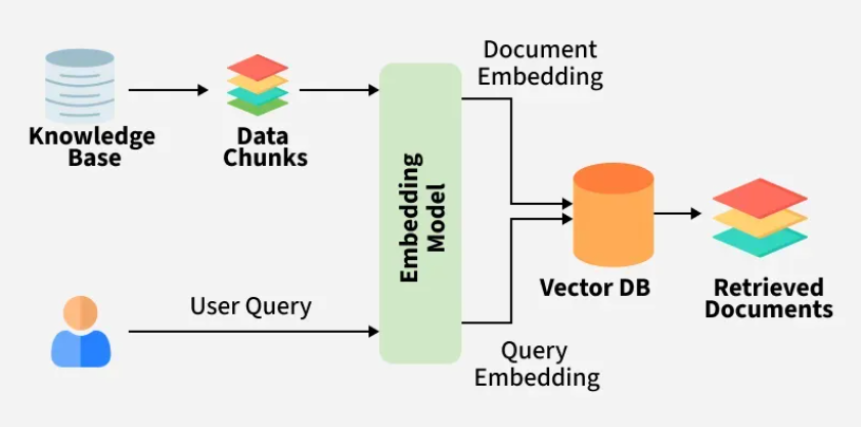
\includegraphics[width=\linewidth]{assets/RAG_1.png}
	\caption{Query processing workflow of the proposed RAG system.}
	\label{fig:rag_workflow}
\end{figure}

The workflow consists of the following steps:

\begin{enumerate}
	\item User submits a medical question.
	\item Query is forwarded to the FastAPI backend.
	\item Query embedding is generated.
	\item FAISS retrieves the most relevant document chunks.
	\item Retrieved context is assembled.
	\item Context and user query are passed to Qwen 2.5.
	\item The language model generates a grounded response.
	\item Source metadata is attached.
	\item Final response is returned to the user.
\end{enumerate}

\subsection{Source Attribution and Explainability}

One of the most important characteristics of the proposed RAG implementation is transparency.

Rather than generating answers without justification, the system preserves metadata associated with retrieved documents and returns source references alongside generated responses. This allows users to trace the origin of information and verify the supporting evidence used during answer generation. The underlying report emphasizes that retrieved documents and page references are preserved to improve transparency and user trust.

Providing source-aware responses is particularly important in healthcare applications where explainability and evidence-based recommendations are essential.

\subsection{Advantages of the Proposed Approach}

The implemented Retrieval-Augmented Generation model provides several advantages:

\begin{itemize}
	\item Reduces hallucinations compared with standalone LLMs.
	\item Produces responses grounded in medical knowledge sources.
	\item Supports explainable and source-aware answers.
	\item Enables efficient retrieval through FAISS vector search.
	\item Preserves privacy through local deployment using Ollama.
	\item Can be continuously expanded by adding new medical documents.
	\item Integrates seamlessly with the overall X-Fed Neuroscan architecture.
\end{itemize}

Consequently, the RAG subsystem serves as an intelligent medical assistant that complements the image analysis capabilities of the platform by providing users with reliable, contextualized, and explainable healthcare information.
